% `template.tex', a bare-bones example employing the AIAA class.
%
% For a more advanced example that makes use of several third-party
% LaTeX packages, see `advanced_example.tex', but please read the
% Known Problems section of the users manual first.
%
% Typical processing for PostScript (PS) output:
%
%  latex template
%  latex template   (repeat as needed to resolve references)
%
%  xdvi template    (onscreen draft display)
%  dvips template   (postscript)
%  gv template.ps   (onscreen display)
%  lpr template.ps  (hardcopy)
%
% With the above, only Encapsulated PostScript (EPS) images can be used.
%
% Typical processing for Portable Document Format (PDF) output:
%
%  pdflatex template
%  pdflatex template      (repeat as needed to resolve references)
%
%  acroread template.pdf  (onscreen display)
%
% If you have EPS figures, you will need to use the epstopdf script
% to convert them to PDF because PDF is a limmited subset of EPS.
% pdflatex accepts a variety of other image formats such as JPG, TIF,
% PNG, and so forth -- check the documentation for your version.
%
% If you do *not* specify suffixes when using the graphicx package's
% \includegraphics command, latex and pdflatex will automatically select
% the appropriate figure format from those available.  This allows you
% to produce PS and PDF output from the same LaTeX source file.
%
% To generate a large format (e.g., 11"x17") PostScript copy for editing
% purposes, use
%
%  dvips -x 1467 -O -0.65in,0.85in -t tabloid template
%
% For further details and support, read the Users Manual, aiaa.pdf.


% Try to reduce the number of latex support calls from people who
% don't read the included documentation.
%


\typeout{}\typeout{If latex fails to find aiaa-tc, read the README file!}
%


\documentclass[]{aiaa-tc}% insert '[draft]' option to show overfull boxes
\usepackage{float}
\usepackage{epstopdf}
\usepackage{amsmath}
\usepackage[table,xcdraw]{xcolor}

\title{Advanced Astrodynamics HW4}

\author{
	Johnathan Clouse%
	\thanks{Graduate Student, Aerospace Engineering Sciences, 1111 Engineering Drive, Boulder, CO, 80309-0429}\\
	{\normalsize\itshape
		University of Colorado, Boulder, CO, 80309-0429, USA}
}

% Define commands to assure consistent treatment throughout document
\newcommand{\eqnref}[1]{(\ref{#1})}
\newcommand{\class}[1]{\texttt{#1}}
\newcommand{\package}[1]{\texttt{#1}}
\newcommand{\file}[1]{\texttt{#1}}
\newcommand{\BibTeX}{\textsc{Bib}\TeX}

\usepackage[euler]{textgreek}
\usepackage[colorlinks=true]{hyperref}
\hypersetup{urlcolor=cyan}

\usepackage{listings}
\usepackage{color} %red, green, blue, yellow, cyan, magenta, black, white
\definecolor{mygreen}{RGB}{28,172,0} % color values Red, Green, Blue
\definecolor{mylilas}{RGB}{170,55,241}

\usepackage{tablefootnote}
\usepackage{graphicx}
\usepackage{amsmath}
\usepackage{bm}
\usepackage{subfigure}
%\usepackage{subcaption}

\definecolor{mylilas}{RGB}{170,55,241}

% See p.105 of "TeX Unbound" for suggested values.
% See pp. 199-200 of Lamport's "LaTeX" book for details.
%   General parameters, for ALL pages:
\renewcommand{\topfraction}{0.9}	% max fraction of floats at top
\renewcommand{\bottomfraction}{0.8}	% max fraction of floats at bottom
%   Parameters for TEXT pages (not float pages):
\setcounter{topnumber}{2}
\setcounter{bottomnumber}{2}
\setcounter{totalnumber}{4}     % 2 may work better
\setcounter{dbltopnumber}{2}    % for 2-column pages
\renewcommand{\dbltopfraction}{0.9}	% fit big float above 2-col. text
\renewcommand{\textfraction}{0.07}	% allow minimal text w. figs
%   Parameters for FLOAT pages (not text pages):
\renewcommand{\floatpagefraction}{0.7}	% require fuller float pages
% N.B.: floatpagefraction MUST be less than topfraction !!
\renewcommand{\dblfloatpagefraction}{0.7}	% require
    \makeatletter
    \renewcommand\l@section{\@dottedtocline{2}{1.5em}{3em}}
    \makeatother
    
\begin{document}
	

	
	\maketitle
	
	\begin{abstract}
		\noindent 
		
	\end{abstract}
	
	\newpage
	
	\tableofcontents
	
	\newpage
	\section{Problem 16: Problem Formulation}
For a Newtonian formulation of the CR3BP, one may take the N-body problem in an inertial frame and set N = 3:
\begin{equation}
\begin{aligned}
m_i\mathbf{\ddot{r}}_i &= -\sum_{j=0,j\neq i}^{3}\frac{Gm_im_j}{r_{ji}^3}\mathbf{r}_{ji}\\
n&=1,2,3\\
\mathbf{r}_{ji}&=\mathbf{r}_{i}-\mathbf{r}_{j}
 \end{aligned}
\end{equation}
where $G$ is the gravitational constant, $m_i$ is the mass of the $i$th body, and $\mathbf{r}_i$ is the position vector of body $i$ in an inertial frame. The primary body is $i=1$, the smaller, secondary body is $i=2$, and the yet-smaller orbiter is $i=3$.By using the convention $m_1>m_2>>m_3$, the following equations of motion can be found:
\begin{equation}
\mathbf{\ddot{r}}_1 = -\frac{Gm_2}{r_{21}^3}\mathbf{r}_{21}
\end{equation}
\begin{equation}
\mathbf{\ddot{r}}_2 = -\frac{Gm_1}{r_{12}^3}\mathbf{r}_{12}
\end{equation}
\begin{equation}
\mathbf{\ddot{r}}_3 = -\frac{Gm_1}{r_{13}^3}\mathbf{r}_{13} -\frac{Gm_2}{r_{23}^3}\mathbf{r}_{23}
\end{equation}
Using this formulation, it is required to integrate the primary and secondary bodies' movement in order to solve for the third body's motion.


The Lagrantian of a system is the sum of the kinetic energy and force potential $U$:
\begin{equation}
L = \frac{1}{2}\mathbf{\dot{r}}_I\cdot \mathbf{\dot{r}}_I +U
\end{equation}
where $U$ for a barycentric system is

\begin{equation}
U=\frac{GM_1}{\left | \mathbf{r}+\nu \boldsymbol{\mathbf{R}} \right |} + \frac{GM_2}{\left | \mathbf{r}-\left (1-\nu  \right ) \boldsymbol{\mathbf{R}} \right |}
\end{equation}
\begin{equation}
\nu=\frac{M_2}{M_1+M_2}
\end{equation}
and $\mathbf{R}$ is the vector from the primary body to the secondary body. 

A coordinate system is chosen to be a constantly-rotating frame where the line between the primary and secondary bodies lies only on the x axis; the origin is the system barycenter. For a circular orbit of the secondary body, both the primary and secondary bodies are stationary in this rotating frame. The velocity can be transformed to inertial coordinates by

\begin{equation}
\mathbf{\dot{r}}_{I}=\mathbf{\dot{r}}_{R}+\boldsymbol{\omega}\times \mathbf{r}_{R} 
\end{equation}
and $\mathbf{R}$ lies solely in x.

With the new rotating coordinate frame, the Lagrangian is now

\begin{equation}
L=\frac{1}{2}\left [ \mathbf{\dot{r}}_R\cdot \mathbf{\dot{r}}_R + \left ( \boldsymbol{\omega} \times \mathbf{r} \right ) \cdot \left ( \boldsymbol{\omega} \times \mathbf{r} \right ) +2\mathbf{\dot{r}}_R \cdot \left (  \boldsymbol{\omega} \times \mathbf{r} \right )\right ] +U
\end{equation}
In scalar form, the Lagrangian is represented as

\begin{equation}
\begin{aligned} 
L=&\frac{1}{2}\left [ \dot{x}+\dot{y}+\dot{z}+ n^2y^2+n^2x^2 +2(-ny\dot{x}+nx\dot{y})\right ]\\&+\frac{GM_1}{\sqrt{x^2+2\nu Rx+\nu^2R^2+y^2+z^2}} + \frac{GM_2}{\sqrt{x^2-2(1-\nu) Rx+(1-\nu)^2R^2+y^2+z^2}}
\end{aligned}
\end{equation}


The Lagrangian equations of motion are given by 
\begin{equation}
\frac{\mathrm{d} }{\mathrm{d} t}\left ( \frac{\partial L}{\partial \mathbf{\dot{q}}} \right ) = \frac{\partial L}{\partial \mathbf{q}}
\end{equation}
where the general coordinates are
\begin{equation}
\mathbf{q}=\mathbf{r}=
\begin{bmatrix}
x\\y\\z
\end{bmatrix}
\end{equation}
\begin{equation}
\mathbf{\dot{q}}=\mathbf{\dot{r}}=
\begin{bmatrix}
\dot{x}\\
\dot{y}\\
\dot{z}
\end{bmatrix}
\end{equation}

Taking the partials with respect to $\mathbf{q}$ and $\mathbf{\dot{q}}$,
\begin{equation}
\frac{\partial L}{\partial \mathbf{q}} =
\begin{aligned}
\frac{\partial L}{\partial {x}} \\ 
\frac{\partial L}{\partial {y}} \\ 
\frac{\partial L}{\partial {z}}
\end{aligned}
=
\begin{aligned} 
 &  xn^2+n\dot{y} - \frac{GM_1}{\left | \mathbf{r}+\nu \boldsymbol{\mathbf{R}}  \right |^3} \left ( x+\nu R \right ) - \frac{GM_2}{\left | \mathbf{r}-\left (1-\nu  \right ) \boldsymbol{\mathbf{R}} \right |^3}\left ( x-(1-\nu)R \right ) \\
& yn^2-n\dot{x} - \frac{GM_1}{\left | \mathbf{r}+\nu \boldsymbol{\mathbf{R}}  \right |^3}  y  - \frac{GM_2}{\left | \mathbf{r}-\left (1-\nu  \right ) \boldsymbol{\mathbf{R}} \right |^3} y \\
 & - \frac{GM_1}{\left | \mathbf{r}+\nu \boldsymbol{\mathbf{R}}  \right |^3}  z - \frac{GM_2}{\left | \mathbf{r}-\left (1-\nu  \right ) \boldsymbol{\mathbf{R}} \right |^3} z
\end{aligned}
\end{equation}

\begin{equation}
\frac{\partial L}{\partial \mathbf{\dot{q}}} =
\begin{aligned}
&\frac{\partial L}{\partial \dot{x}} && \dot{x}-ny\\ 
&\frac{\partial L}{\partial \dot{y}} =&& \dot{y}+nx\\ 
&\frac{\partial L}{\partial \dot{z}} && \dot{z}
\end{aligned}
\end{equation}
The equations of motion in the barycentric rotating frame using the Lagrangian formulation is:
\begin{equation}
\ddot{q}=\begin{bmatrix}
\ddot{x}\\ 
\ddot{y}\\ 
\ddot{z}
\end{bmatrix}
=
\begin{bmatrix}
xn^2+n\dot{y} - \frac{GM_1}{\left | \mathbf{r}+\nu \boldsymbol{\mathbf{R}}  \right |^3} \left ( x+\nu R \right ) - \frac{GM_2}{\left | \mathbf{r}-\left (1-\nu  \right ) \boldsymbol{\mathbf{R}} \right |^3}\left ( x-(1-\nu)R \right ) +n\dot{y}\\ 
yn^2-n\dot{x} - \frac{GM_1}{\left | \mathbf{r}+\nu \boldsymbol{\mathbf{R}}  \right |^3}  y  - \frac{GM_2}{\left | \mathbf{r}-\left (1-\nu  \right ) \boldsymbol{\mathbf{R}} \right |^3} y-n\dot{x}\\ 
- \frac{GM_1}{\left | \mathbf{r}+\nu \boldsymbol{\mathbf{R}}  \right |^3}  z - \frac{GM_2}{\left | \mathbf{r}-\left (1-\nu  \right ) \boldsymbol{\mathbf{R}} \right |^3} z
\end{bmatrix}
\end{equation}

The Jacobi integral for the Lagrangian is given by
\begin{equation}
J=\frac{\partial L}{\partial \mathbf{\dot{q}}}\cdot \mathbf{\dot{q}}-L
\label{eqn:Jacobi}
\end{equation}
For this circular, rotating, barycentric system, the constant Jacobi integral is 
\begin{equation}
\begin{aligned}
J &= \dot{x}^2-ny\dot{x}+\dot{y}^2+nx\dot{y}+\dot{z}^2 -L\\ 
 &= \mathbf{\dot{r}}_R \cdot \mathbf{\dot{r}}_R+2\mathbf{\dot{r}}_R\cdot(\boldsymbol{\omega }\times \mathbf{r}) - \frac{1}{2}\left [ \mathbf{\dot{r}}_R\cdot \mathbf{\dot{r}}_R + \left ( \boldsymbol{\omega} \times \mathbf{r} \right ) \cdot \left ( \boldsymbol{\omega} \times \mathbf{r} \right ) +2\mathbf{\dot{r}}_R \cdot \left (  \boldsymbol{\omega} \times \mathbf{r} \right )\right ] -U\\
 &= \frac{1}{2}\mathbf{\dot{r}}_R \cdot \mathbf{\dot{r}}_R- \frac{\left ( \boldsymbol{\omega} \times \mathbf{r} \right ) \cdot \left ( \boldsymbol{\omega} \times \mathbf{r} \right )}{2}  -U
\end{aligned}
\end{equation}

	\section{Problem 16: Simulation verification}	
Numerical integration routines using the Newton and Lagrange formulations were created to study the CR3BP. Some test cases were performed to ensure that the integrators had similar solutions, that the 2-body orbit elements were constant when $M_2$ = 0 (except true anomaly), and that the Jacobi integral was conserved. Table \ref{tbl:OrbitCharacteristics}
\begin{table}[H]
\centering
\caption{Orbit characteristics}
\label{tbl:OrbitCharacteristics}
\begin{tabular}{|l|l|}
\hline
\rowcolor[HTML]{C0C0C0} 
\textbf{Parameter} & \textbf{Value} \\ \hline
$M_1$                  &  5.9742e+24 kg             \\ \hline
$M_2$                  &  7.3483e+22 kg             \\ \hline
$R$                  &  384400 km             \\ \hline
a                  & 7000 km             \\ \hline
e                  & 0.01           \\ \hline
i                  & 30$^\circ$     \\ \hline
$\Omega$           & 0$^\circ$                \\ \hline
$\omega$           & 45$^\circ$               \\ \hline
\end{tabular}
\end{table}

The percent error between the Newton and Lagrange formulations are shown in Figure \ref{fig:Orb_ex_errors} below:
	\begin{figure}[H]
		\centering
		\subfigure[Position percent error]{
			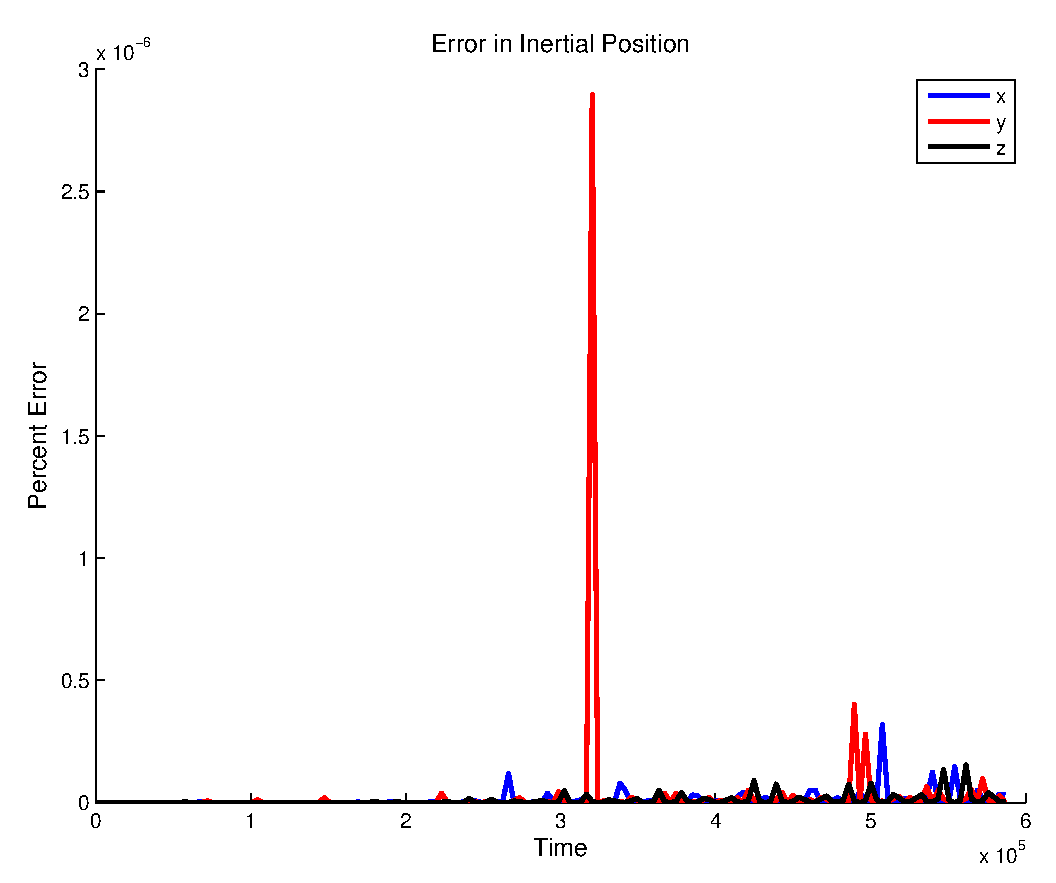
\includegraphics[width = 10cm]{Figures/Pos_Err_Example_Orb.eps}
		}
		\subfigure[Velocity percent error]{
			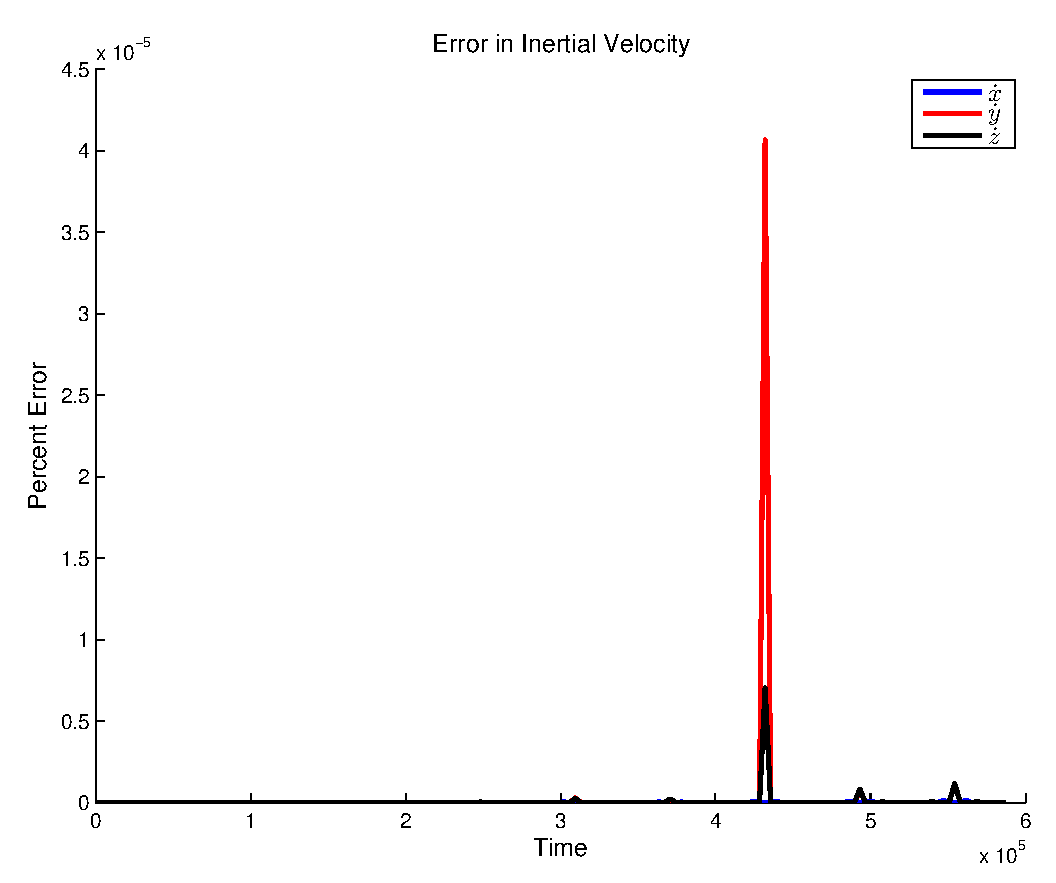
\includegraphics[width = 10cm]{Figures/Vel_Err_Example_Orb.eps}
		}
	\caption{Different integration routines compared. }
		\label{fig:Orb_ex_errors}
	\end{figure}

The Jacobi integral conservation can be seen in Figure \ref{fig:Jacobi_conserved} below:
	\begin{figure}[H]
		\centering
			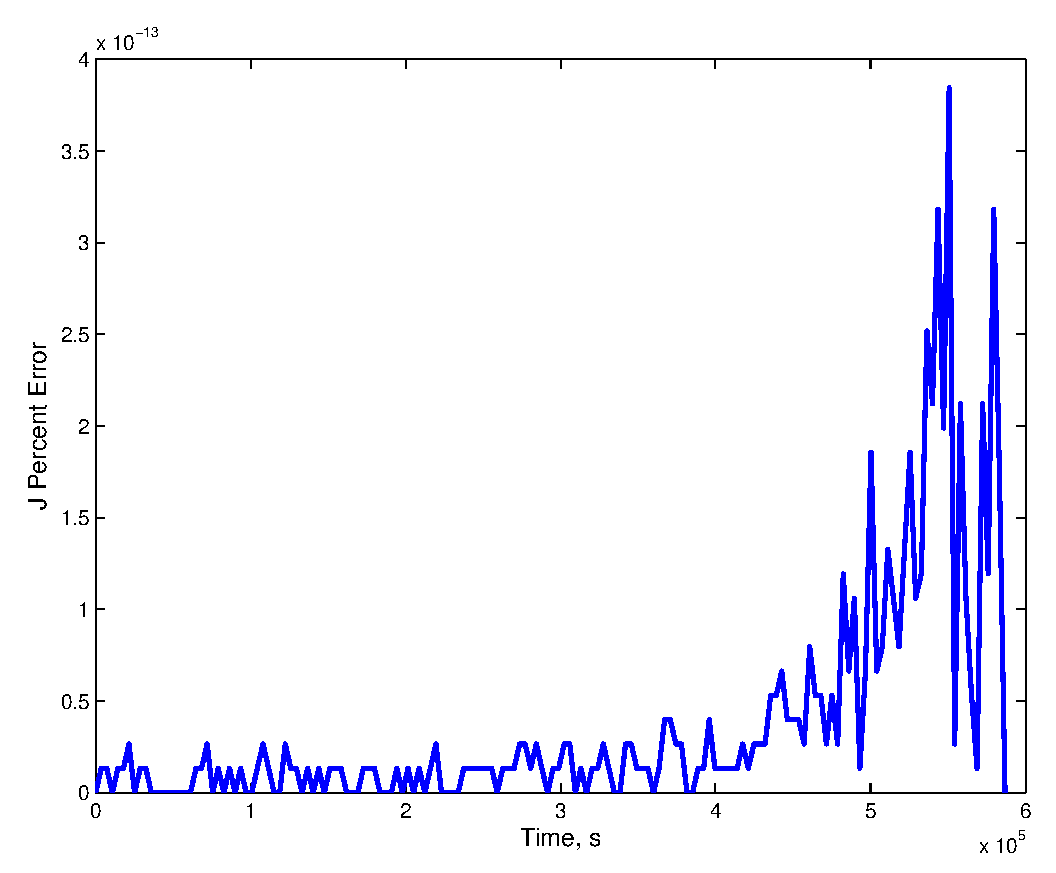
\includegraphics[width = 10cm]{Figures/J_conserved.eps}
	\caption{Conservation of the Jacobi integral. }
		\label{fig:Jacobi_conserved}
	\end{figure}

Figure \ref{fig:Orb_elems_m2_0} shows the orbital elements when $M_2=0$. Figure \ref{fig:Orb_elems_m2_0_err} shows the error from the initial conditions.
	\begin{figure}[H]
		\centering
		\subfigure[a]{
			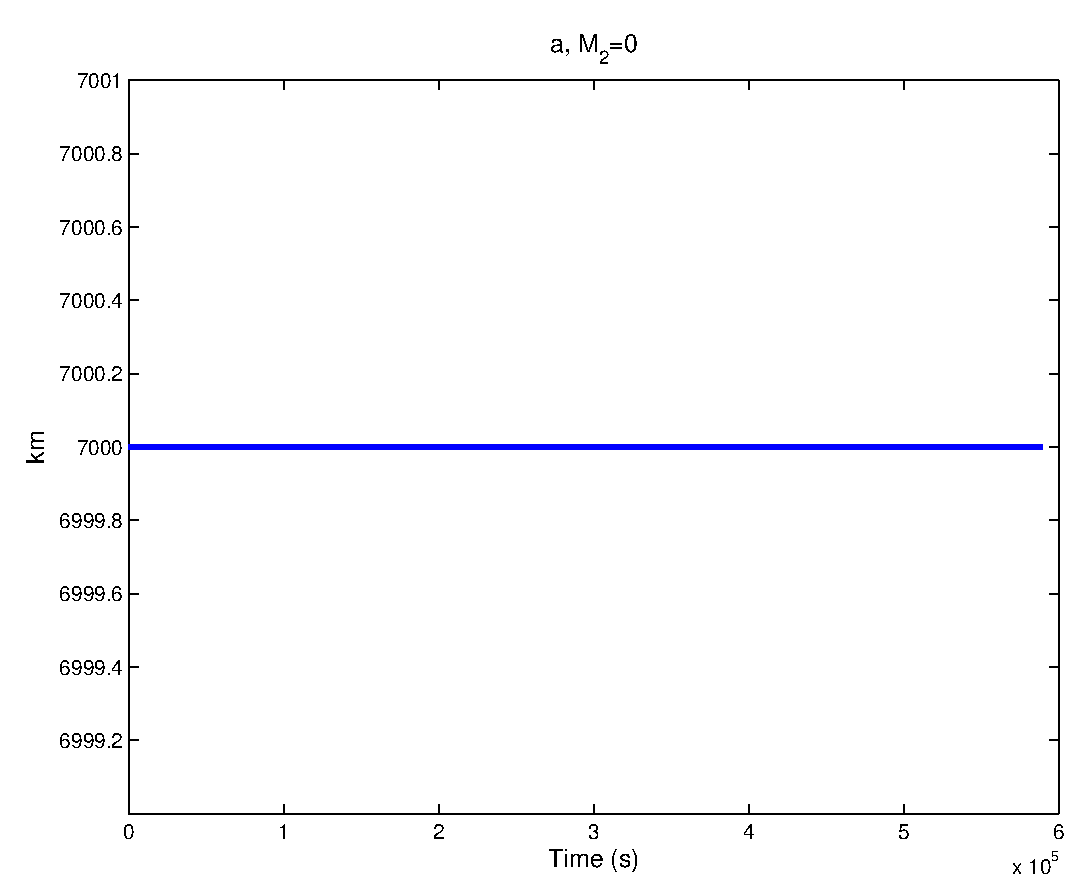
\includegraphics[width = 7.5cm]{Figures/OE_Conserved_a.eps}
		}
		\subfigure[e]{
			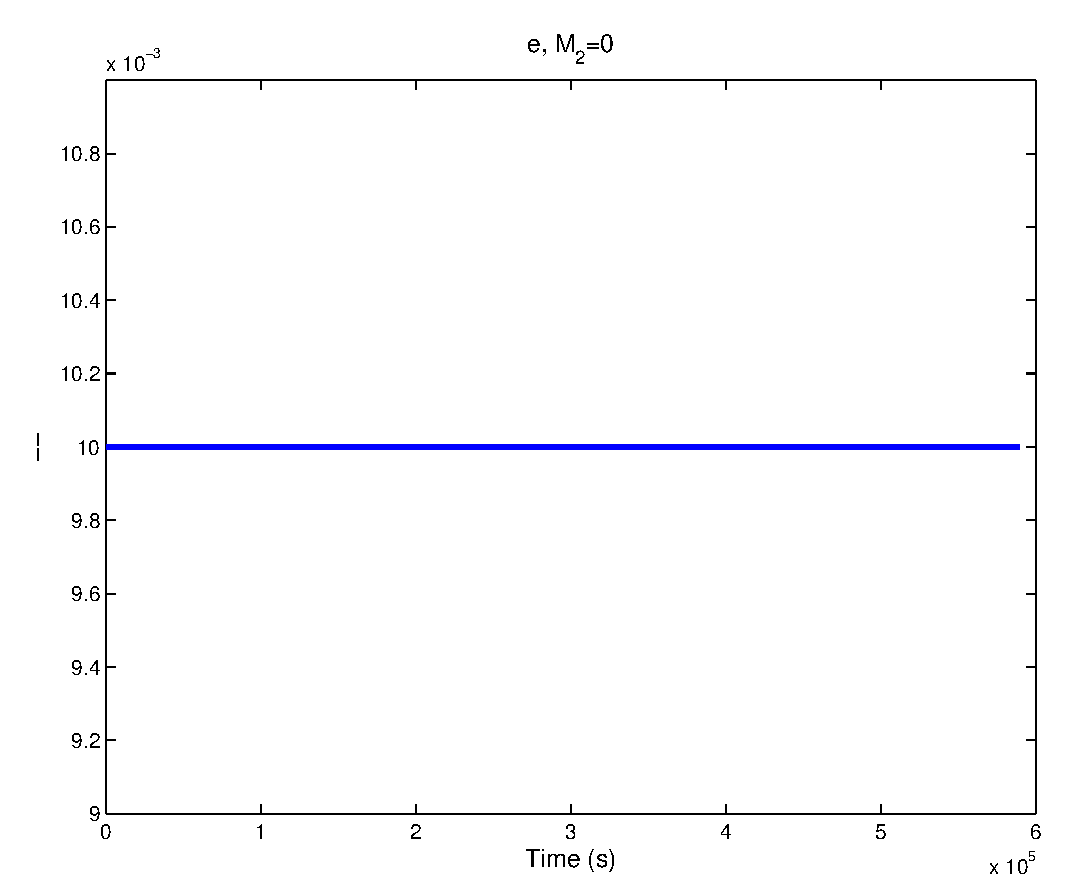
\includegraphics[width = 7.5cm]{Figures/OE_Conserved_e.eps}
		}
		\subfigure[i]{
			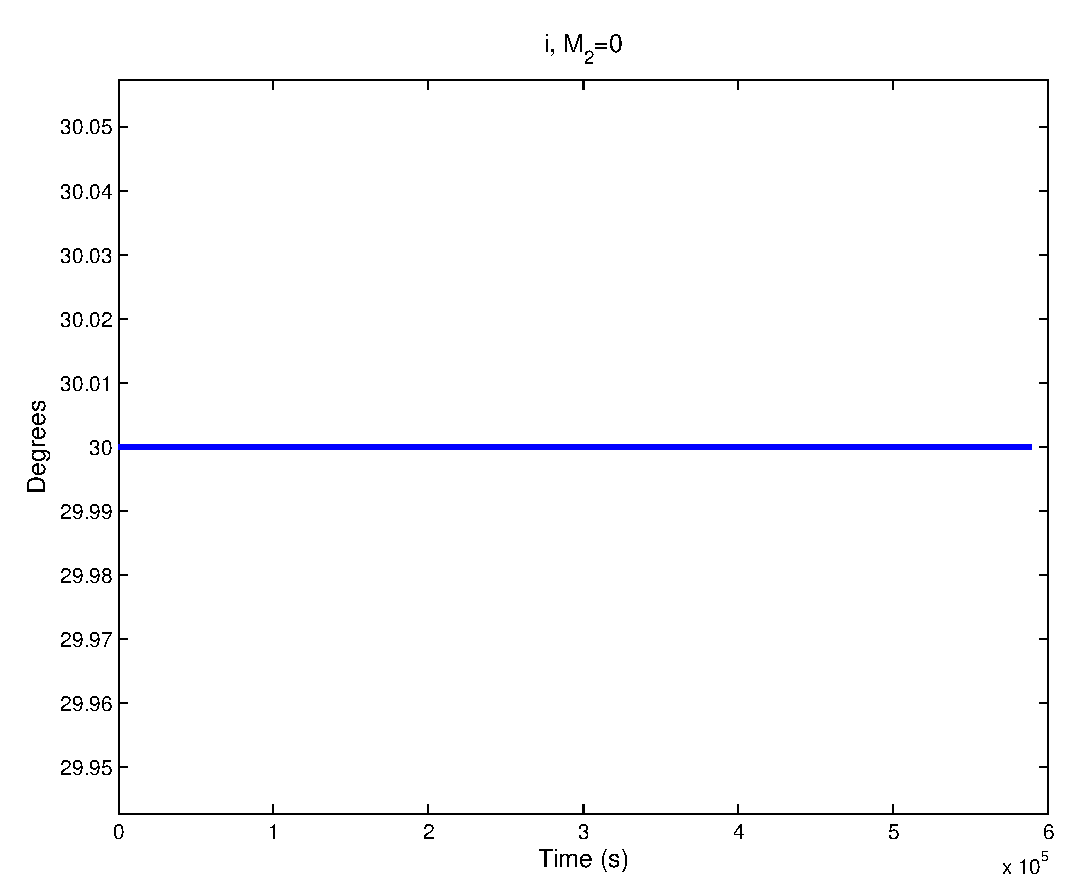
\includegraphics[width = 7.5cm]{Figures/OE_Conserved_i.eps}
		}
		\subfigure[$\Omega$]{
			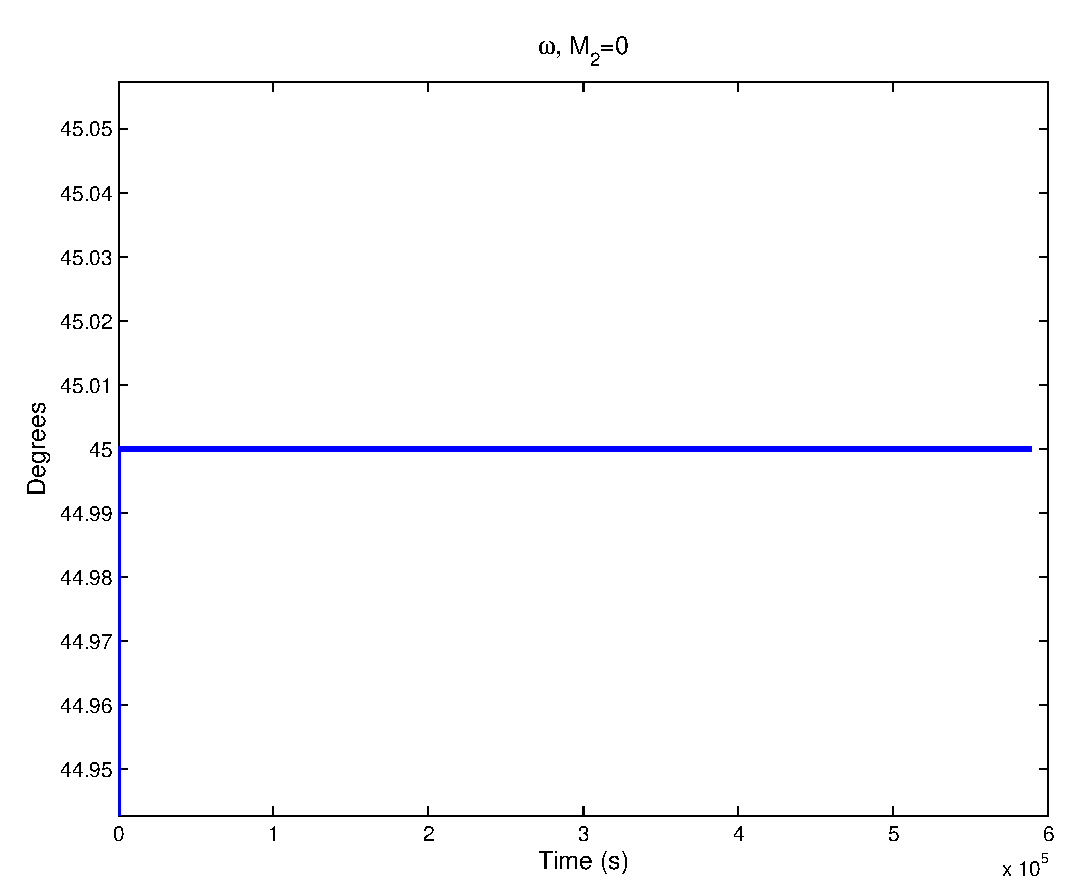
\includegraphics[width = 7.5cm]{Figures/OE_Conserved_W.eps}
		}
		\subfigure[$\omega$]{
			\includegraphics[width = 7.5cm]{Figures/OE_Conserved_w.eps}
		}
	\caption{Numerical integration results when $M_2=0$. }
		\label{fig:Orb_elems_m2_0}
	\end{figure}
	\begin{figure}[H]
		\centering
		\subfigure[a]{
			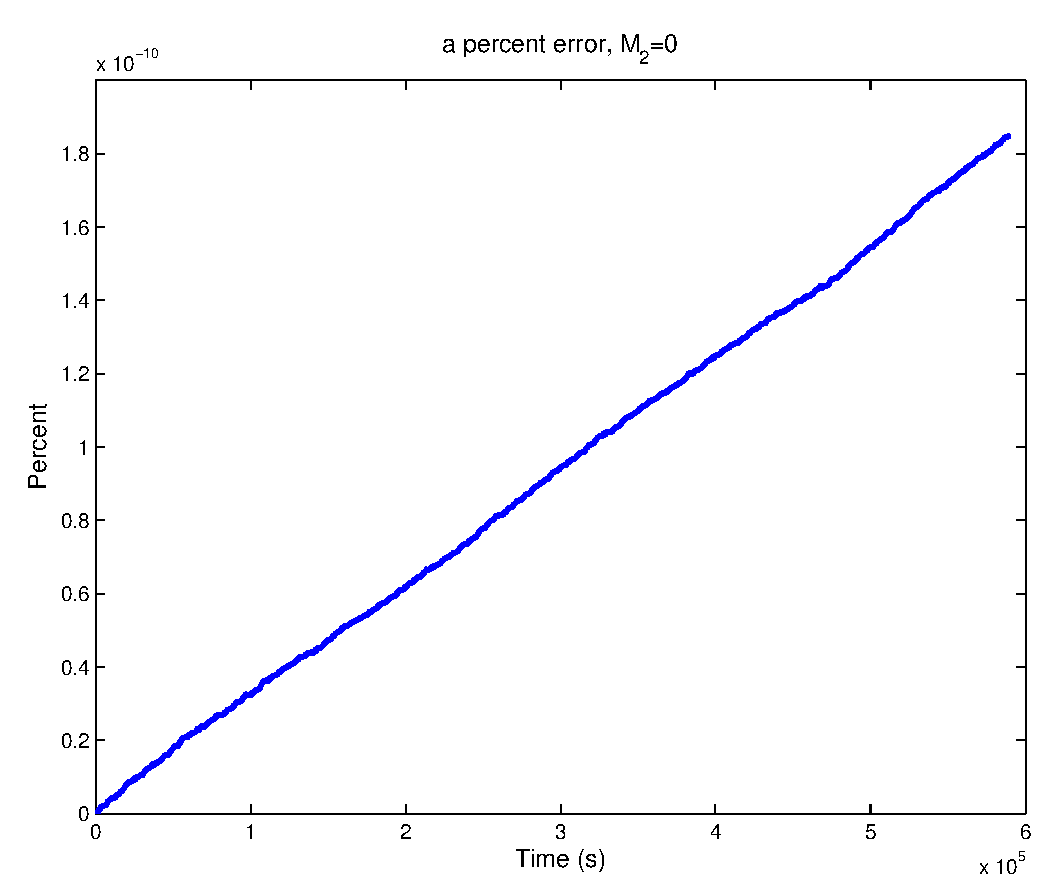
\includegraphics[width = 7.5cm]{Figures/OE_Conserved_a_PE.eps}
		}
		\subfigure[e]{
			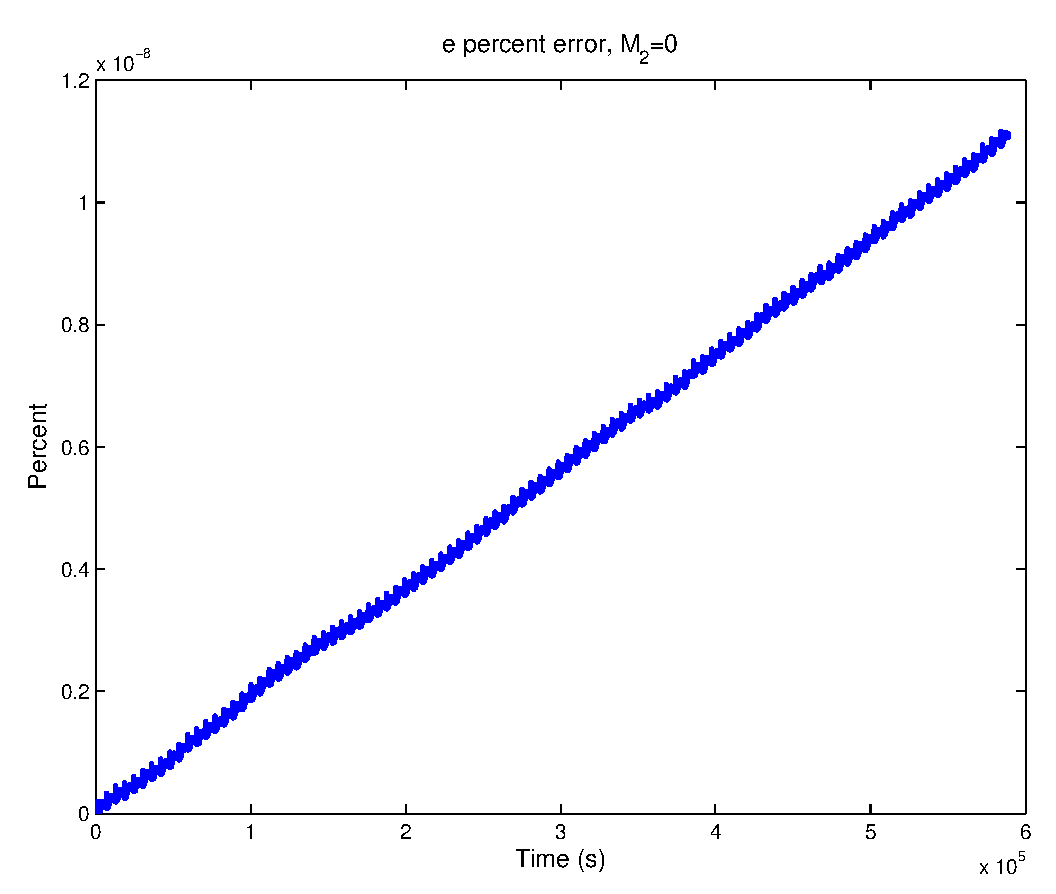
\includegraphics[width = 7.5cm]{Figures/OE_Conserved_e_PE.eps}
		}
		\subfigure[i]{
			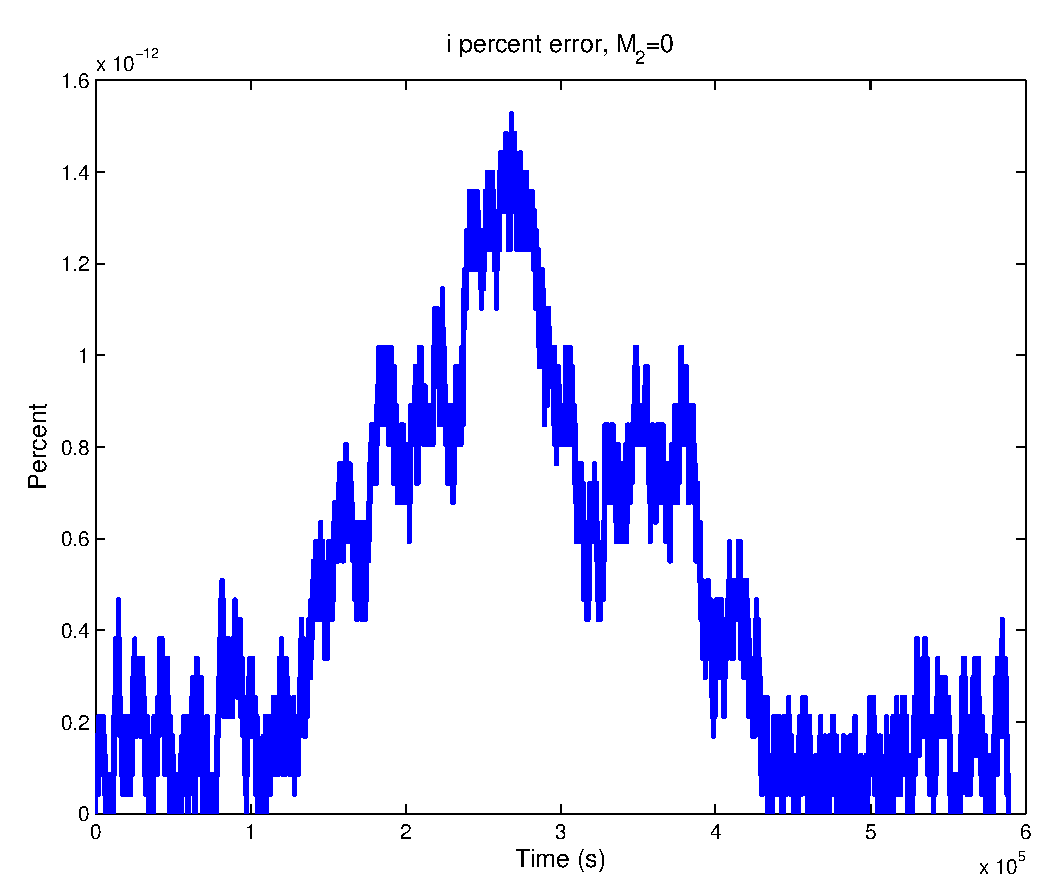
\includegraphics[width = 7.5cm]{Figures/OE_Conserved_i_PE.eps}
		}
		\subfigure[$\Omega$]{
			\includegraphics[width = 7.5cm]{Figures/OE_Conserved_W_PE.eps}
		}
		\subfigure[$\omega$]{
			\includegraphics[width = 7.5cm]{Figures/OE_Conserved_w_PE.eps}
		}
	\caption{Numerical integration errors with initial conditions when $M_2=0$. }
		\label{fig:Orb_elems_m2_0_err}
	\end{figure}

\bibliographystyle{aiaa}   % Number the references.
\bibliography{ASEN6080ProjectBib}   % Use references.bib to resolve the labels.

%    \section{Appendix B}
%This appendix contains all Matlab code used by the authors to analyize their data.
%    
%    \lstset{language=Matlab,%
%    	%basicstyle=\color{red},
%    	breaklines=true,%
%    	morekeywords={matlab2tikz},
%    	keywordstyle=\color{blue},%
%    	morekeywords=[2]{1}, keywordstyle=[2]{\color{black}},
%    	identifierstyle=\color{black},%
%    	stringstyle=\color{mylilas},
%    	commentstyle=\color{mygreen},%
%    	showstringspaces=false,%without this there will be a symbol in the places where there is a space
%    	numbers=left,%
%    	numberstyle={\tiny \color{black}},% size of the numbers
%    	numbersep=9pt, % this defines how far the numbers are from the text
%    	emph=[1]{for,end,break},emphstyle=[1]\color{red}, %some words to emphasise
%    	%emph=[2]{word1,word2}, emphstyle=[2]{style},   
%    }
    
%    \lstinputlisting{ASEN5090_ecef2azelrange.m}
%    \vspace{5mm}
%    
%    \lstinputlisting{ASEN5090_GPSvis.m}
%    \vspace{5mm}
%\lstinputlisting{HW5_rel_err.m}
%\vspace{5mm}
%\lstinputlisting{import_gps_data.m}
%\vspace{5mm}
%\lstinputlisting{datenum8601.m}
%\vspace{5mm}
%\lstinputlisting{lab_err_plots.m}
%\vspace{5mm}
	
\end{document}

% - Release $Name:  $ -
